\section{Дрейф, вызванный изменениями магнитного поля только по числовому значению.}

Для определения мгновенной скорости дрейфа введем локальную систему отсчета, направив ось $Z$ вдоль магнитного поля $\vec{B}$.
Единичный вектор вдоль $\textbf{B}$ обозначим через $\textbf{h}$. 
Направление главной нормали $N$ к магнитной силовой линии примем
за ось \textit{Y}. Ось \textit{X} направим в отрицательную сторону бинормали $\textbf{b}=\textbf{h} \times \textbf{N}$ (рис. \ref{pic199})

\begin{figure}[h!]
    \centering
    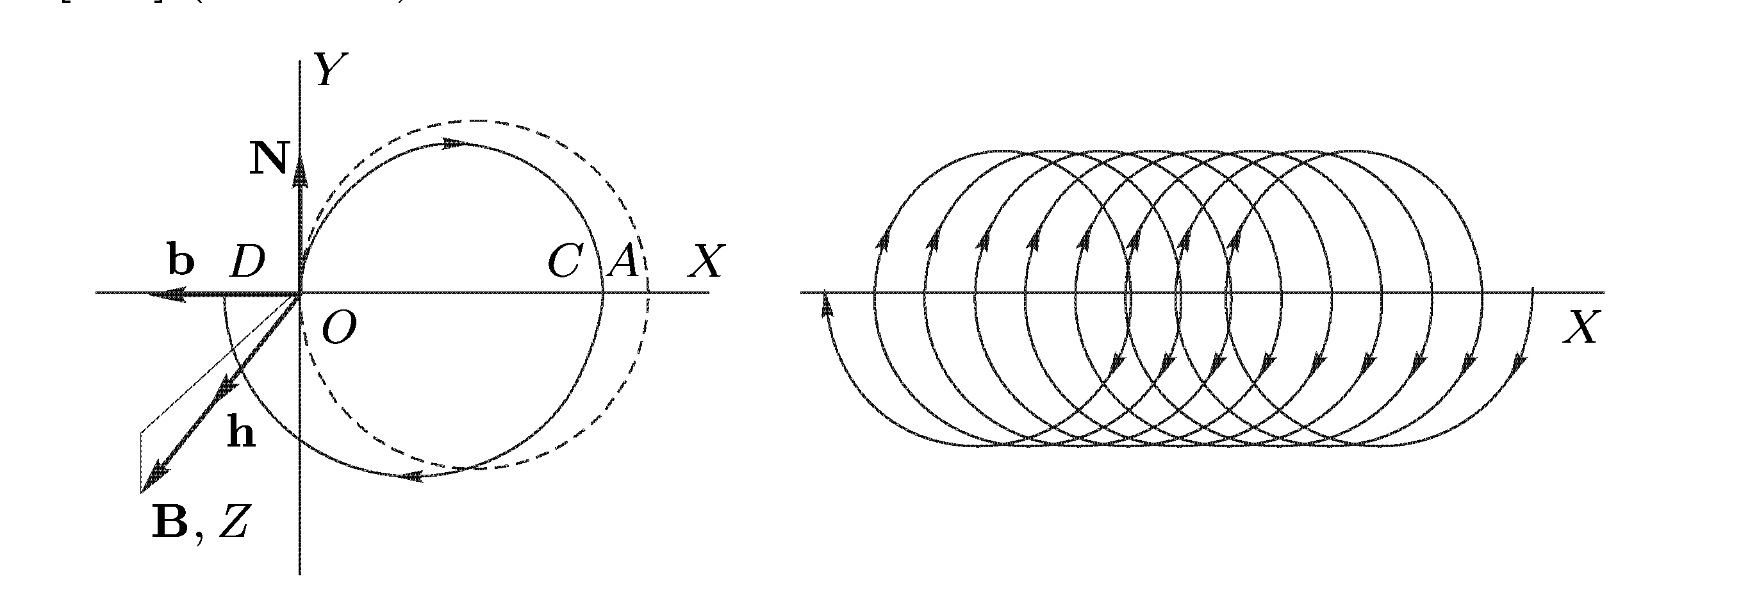
\includegraphics[scale=0.3]{199.png}
    \caption{}
    \label{pic199}
\end{figure}

Максимальное изменение числового значения магнитного поля происходит в направлении главной нормали \textbf{N}. 
В случае, который нас более всего интересует, когда частица движется в области пространства, где не текут электрические токи, поле $\textbf{H} \equiv \textbf{B}$ в направлении \textbf{N} будет возрастать. 
Для доказательства возьмем в соприкасающейся плоскости две бесконечно близкие магнитные силовые линии \textit{BC} и \textit{AD} и два бесконечно коротких отрезка \textit{AB} и \textit{CD}, перпендикулярных к этим силовым линиям (рис. \ref{pic200}). 
Циркуляция вектора \textbf{H} по бесконечномалому контуру \textit{BCDА} будет $H_1 l_1 - H_2 l_2$, где $l_1$ и $l_2$ — длины сторон \textit{BC} и \textit{AD}, а $H_1$ и $H_2$ - напряженности магнитного поля на этих сторонах. 

\begin{figure}[h!]
    \centering
    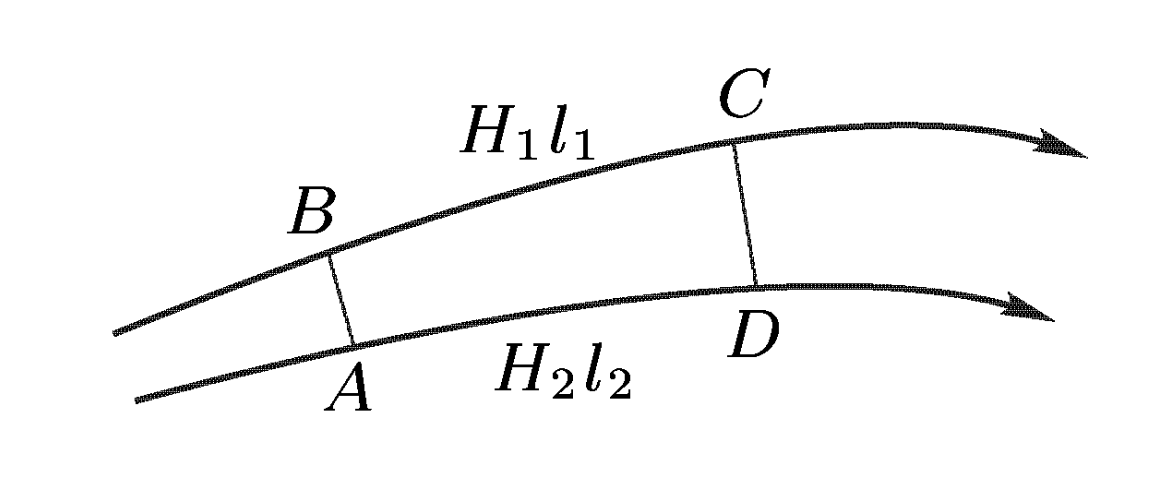
\includegraphics[scale=0.3]{200.png}
    \caption{}
    \label{pic200}
\end{figure}

Так как в отсутствие электрических токов эта циркуляция равна нулю, то магнитное поле $H$ будет больше на более короткой стороне. 

Отсюда и следует наше утверждение.
Сейчас речь идет о влиянии на скорость дрейфа изменения магнитного поля, но не его направления. 
Поэтому можно отвлечься от кривизны магнитных силовых линий и считать их прямолинейными. 
Можно также отвлечься от наличия продольной составляющей скорости $\textbf{v}_{\parallel}$, так как движение вдоль магнитного поля не влияет на силы, действующие на частицу. 
Иными словами, во всех промежуточных расчетах под $\textbf{v}$ следует понимать поперечную скорость $\textbf{v}_{\perp}$. 
Ради краткости опустим всюду значок $\perp$, за исключением окончательных формул, в которых поперечная скорость по-прежнему будет обозначаться через $\textbf{v}_{\perp}$ . 
Кроме того, во всех промежуточных расчетах заряд частицы $e$ будем считать положительным.
Положительно заряженная частица будет вращаться по часовой стрелке, как указано на рис. \ref{pic199}. Выйдя из точки \textit{O}, частица двигалась бы по окружности радиуса $\rho = \textit{v} / \omega_в$, если бы магнитное поле \textbf{B} было постоянно. 
Эта окружность изображена на рис. \ref{pic199} пунктиром. Она пересекает ось \textit{X} в точке \textit{A} на расстоянии \textit{OA} = $2\rho$ от точки \textit{O}. 
В действительности магнитное поле, а с ним и кривизна траектории возрастают с возрастанием координаты \textit{y}. 
Поэтому частица вернется к оси \textit{X} в какой-то точке \textit{C}, расположенной левее \textit{A}. 
При движении в нижней половине плоскости \textit{XY}, наоборот, кривизна траектории будет меньше, а потому частица пересечет ось \textit{X} в точке \textit{D}, расположенной левее \textit{O}. 
Таким образом, за один оборот положительно заряженная частица сместится влево на отрезок \textit{OD}.
Отрицательно заряженная частица сместилась бы в противоположном направлении. 
При медленном изменении магнитного поля в пространстве траектория частицы за один оборот мало отличается от окружности, и смещение \textit{OD} будет мало по сравнению с радиусом $\rho$. 
Путь частицы за время многих оборотов изображен на рис. \ref{pic199} справа.
Частица быстро вращается по окружности, центр которой медленно перемещается параллельно оси \textit{X}. 
Такое перемещение и есть дрейф. 

Найдем теперь скорость дрейфа $v_д$, усреднив движение частицы по быстрому ларморовскому вращению. 
Уравнение движения частицы $\dot{\textbf{v}} = \left[ \textbf{v} \omega_B \right]$ запишем в координатной форме:

\begin{equation*}
    \dot v_x  = v_y \cdot \omega_в, ~~~ \dot v_y = -v_x \cdot \omega_в
\end{equation*}

Поскольку дрейф происходит параллельно оси \textit{X} и отсутствует в направлении оси \textit{Y}, скорость дрейфа $v_д = \overline{v}_x$ найдется из требования, что среднее значение $v_y$, а следовательно, и $\dot v_y = -v_x \cdot \omega_в$ равно нулю, т.е. $\overline{v_x \cdot \omega_в} = 0$. Разложим $\omega_в$ в ряд по степеням $y$ и оборвем это разложение на линейном члене:

\begin{equation*}
    \omega_в = \omega_0 + \left( \dfrac{d\omega_в}{dy} \right)_{y=0} y.
\end{equation*}
Тогда:

\begin{equation*}
    \overline{v}_x \cdot \omega_0 + \dfrac{d\omega_в}{dy} \overline{y \cdot v_x} = 0.
\end{equation*}

Так как величина $\dfrac{d\omega_в}{dy}$ предполагается малой, то среднее значение произведения $y \cdot v_x = y \cdot \dot x$ достаточно вычислить в нулевом приближении, т.~е. считать при вычислении, что частица вращается по окружности

\begin{equation*}
    x = \rho \cos \left( \omega_0 \cdot t \right), ~~~y = - \rho \sin \left( \omega_0 \cdot t \right)
\end{equation*}

Тогда:

\begin{equation*}
    \overline{y \cdot \dot x} = \rho^2 \omega_0 \cdot \overline{\sin^2 \omega_0 t} = \dfrac{\rho^2 \omega_0}{2}
\end{equation*}

и следовательно,

\begin{equation*}
    v_д = \overline{v}_x = -\dfrac{\rho^2}{2} \dfrac{d\omega_в}{dy}
\end{equation*}

В векторной форме:

\begin{equation}
    \label{formula_41}
    \textbf{v}_д = \dfrac{\rho^2}{2} \dfrac{d\omega_в}{dy} \textbf{b}
\end{equation}

или с учетом соотношений $\rho = \dfrac{v}{\omega_в}$ и $\omega_в = \dfrac{eB}{mc}$

\begin{equation}
    \label{formula_42}
    \textbf{v}_д = \dfrac{mcv^2_{\perp}}{2eB^2} \dfrac{\partial B}{\partial N} \textbf{b}
\end{equation}

В этом виде формула верна и для положительно заряженной, и для отрицательно заряженной частицы. Положительно заряженная частица дрейфует в положительном направлении бинормали к магнитной силовой линии, отрицательно заряженная — в отрицательном направлении.
Придадим теперь формуле (\ref{formula_42}) более наглядную геометрическую форму, предполагая, что пространство, в котором движется частица, свободно от электрических токов. 
Имея в виду, что поле \textbf{B} в рассматриваемой точке направлено вдоль оси \textit{Z}, запишем формулу (\ref{formula_42}) в виде

\begin{equation*}
    \textbf{v}_д = \dfrac{mcv^2_{\perp}}{2eB^2} \dfrac{\partial B_z}{\partial y} \textbf{b}
\end{equation*}

Так как при отсутствии электрических токов $rot B = 0$, то $\dfrac{\partial B_z}{\partial y} = \dfrac{\partial B_y}{\partial z}$, и, следовательно,

\begin{equation*}
    \textbf{v}_д = \dfrac{mcv^2_{\perp}}{2eB^2} \dfrac{\partial B_y}{\partial z} \textbf{b}
\end{equation*}

Как видно из рис. \ref{pic201}, $\tan \alpha = \dfrac{B_y}{B_z}$, где $\alpha$ — угол между касательной к магнитной силовой линии и осью \textit{Z}. 
В начале координат \textit{O} касательная горизонтальна, а потому в его малой окрестности $\tan \alpha$ можно заменить на $\alpha$. 

\begin{figure}
    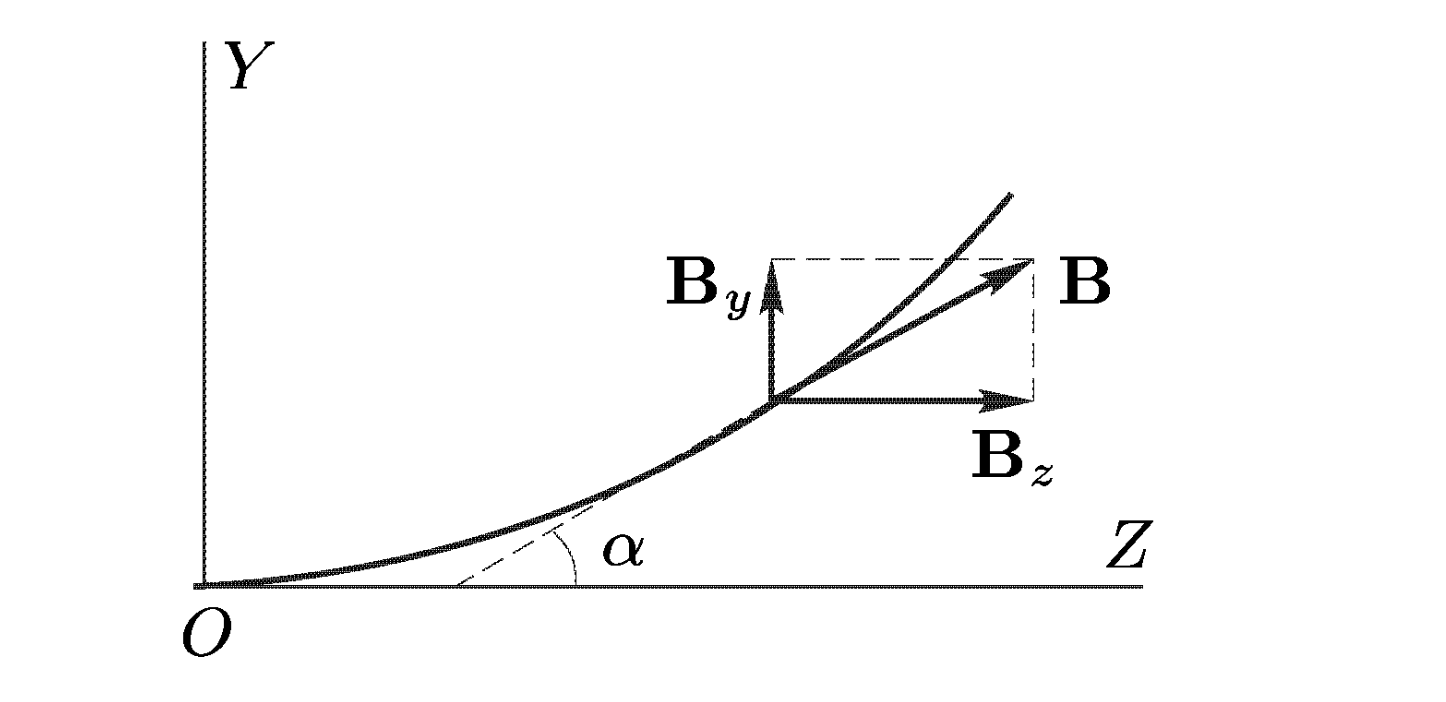
\includegraphics[scale=0.3]{201.png}
    \centering
    \caption{}
    \label{pic201}
\end{figure}

По той же причине дифференцирование по дуге магнитной силовой линии можно заменить дифференцированием по координате $z$.

Радиус кривизны $R$ силовой линии определяется соотношением

\begin{equation*}
    \dfrac{1}{R} = \dfrac{d\alpha}{ds} = \dfrac{\partial}{\partial z} \left( \dfrac{B_y}{B_z} \right) = \dfrac{1}{B_z} \dfrac{\partial B_y}{\partial z} - \dfrac{B_y}{B_z^2} \dfrac{\partial B_z}{\partial z}, ~\text{или}~ \dfrac{1}{R} = \dfrac{1}{B} \dfrac{\partial B_y}{\partial z}
\end{equation*}

так как в точке \textit{O} $B_z = B$, $B_y = 0$. B результате получается

\begin{equation}
    \label{formula_43}
    \textbf{v}_д = \dfrac{mcv^2_{\perp}}{2eBR} \textbf{b}
\end{equation}
